% Petri net "Order processing", generated by pnm
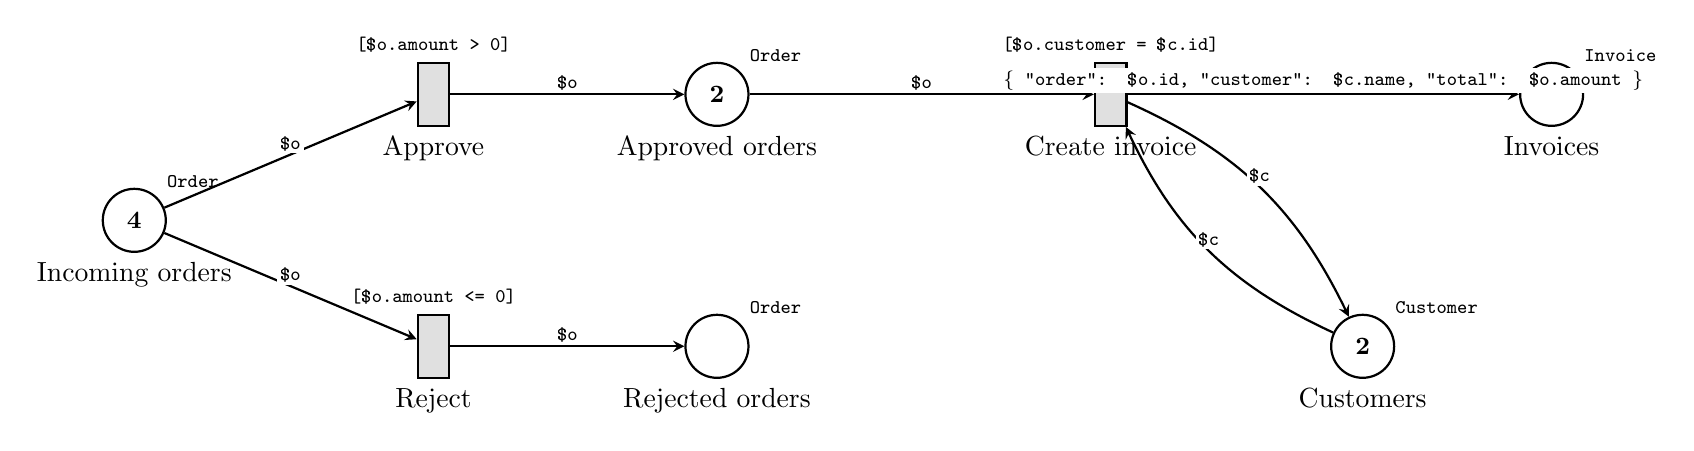
\begin{tikzpicture}
  \tikzset{
    place/.style={circle, draw=black, fill=white, thick, minimum size=8mm, inner sep=0pt},
    transition/.style={rectangle, draw=black, fill=black!12, thick, minimum width=4mm, minimum height=8mm, inner sep=0pt},
    arc/.style={->, >=stealth, thick},
    token/.style={circle, fill=black, inner sep=1.2pt},
  }
  % Places
  \node[place, label={below:{Incoming orders}}, label={[font=\scriptsize]above right:{\texttt{Order}}}, font=\small\bfseries] (incoming) at (0,1.6) {4};
  \node[place, label={below:{Approved orders}}, label={[font=\scriptsize]above right:{\texttt{Order}}}, font=\small\bfseries] (approved) at (7.4,3.2) {2};
  \node[place, label={below:{Rejected orders}}, label={[font=\scriptsize]above right:{\texttt{Order}}}] (rejected) at (7.4,0) {};
  \node[place, label={below:{Customers}}, label={[font=\scriptsize]above right:{\texttt{Customer}}}, font=\small\bfseries] (customers) at (15.6,0) {2};
  \node[place, label={below:{Invoices}}, label={[font=\scriptsize]above right:{\texttt{Invoice}}}] (invoices) at (18,3.2) {};
  % Transitions
  \node[transition, label={below:{Approve}}, label={[font=\scriptsize]above:{\texttt{[\$o.amount > 0]}}}] (approve) at (3.8,3.2) {};
  \node[transition, label={below:{Reject}}, label={[font=\scriptsize]above:{\texttt{[\$o.amount <= 0]}}}] (reject) at (3.8,0) {};
  \node[transition, label={below:{Create invoice}}, label={[font=\scriptsize]above:{\texttt{[\$o.customer = \$c.id]}}}] (invoice) at (12.4,3.2) {};
  % Arcs
  \draw[arc] (incoming) -- node[midway, above, fill=white, inner sep=1pt, font=\scriptsize] {\texttt{\$o}} (approve);
  \draw[arc] (approve) -- node[midway, above, fill=white, inner sep=1pt, font=\scriptsize] {\texttt{\$o}} (approved);
  \draw[arc] (incoming) -- node[midway, above, fill=white, inner sep=1pt, font=\scriptsize] {\texttt{\$o}} (reject);
  \draw[arc] (reject) -- node[midway, above, fill=white, inner sep=1pt, font=\scriptsize] {\texttt{\$o}} (rejected);
  \draw[arc] (approved) -- node[midway, above, fill=white, inner sep=1pt, font=\scriptsize] {\texttt{\$o}} (invoice);
  \draw[arc] (customers) to[bend left=20] node[midway, above, fill=white, inner sep=1pt, font=\scriptsize] {\texttt{\$c}} (invoice);
  \draw[arc] (invoice) to[bend left=20] node[midway, above, fill=white, inner sep=1pt, font=\scriptsize] {\texttt{\$c}} (customers);
  \draw[arc] (invoice) -- node[midway, above, fill=white, inner sep=1pt, font=\scriptsize] {\texttt{\{ "order": \$o.id, "customer": \$c.name, "total": \$o.amount \}}} (invoices);
\end{tikzpicture}
